\documentclass{article}
\usepackage{fontspec}
\setmainfont{Times New Roman}
\usepackage{geometry}
\usepackage{CTEX}
\geometry{papersize={21cm,29.7cm}}
\geometry{left=3.18cm,right=3.18cm,top=2.54cm,bottom=2.54cm}
\usepackage{fancyhdr}
\usepackage{amsmath}
\pagestyle{fancy}
\lhead{学号:202000460020}
\rhead{姓名:苏博南}
\cfoot{\thepage}
\renewcommand{\headrulewidth}{0.4pt}
\renewcommand{\headwidth}{\textwidth}
\usepackage{tikz}
\usetikzlibrary{automata, positioning, arrows}
\usepackage{listings}
\usepackage{float}
\lstset{
	basicstyle=\small\ttfamily,	% 基本样式
		keywordstyle=\color{blue}, % 关键词样式
		commentstyle=\color{gray!50!black!50},   	% 注释样式
		stringstyle=\rmfamily\slshape\color{red}, 	% 字符串样式
	backgroundcolor=\color{gray!0},     % 代码块背景颜色
	frame=leftline,						% 代码框形状
	framerule=12pt,%
		rulecolor=\color{gray!0},      % 代码框颜色
	numbers=left,				% 左侧显示行号往左靠, 还可以为right ,或none,即不加行号
		numberstyle=\footnotesize\itshape,	% 行号的样式
		firstnumber=1,
		stepnumber=1,                  	% 若设置为2,则显示行号为1,3,5
		numbersep=7pt,               	% 行号与代码之间的间距
	aboveskip=.25em, 			% 代码块边框
	showspaces=false,               	% 显示添加特定下划线的空格
	showstringspaces=false,         	% 不显示代码字符串中间的空格标记
	keepspaces=true, 					
	showtabs=false,                 	% 在字符串中显示制表符
	tabsize=2,                     		% 默认缩进2个字符
	captionpos=b,                   	% 将标题位置设置为底部
	flexiblecolumns=true, 			%
	breaklines=true,                	% 设置自动断行
	breakatwhitespace=false,        	% 设置自动中断是否只发生在空格处
	breakautoindent=true,			%
	breakindent=1em, 			%
	title=\lstname,				%
	escapeinside=``,  			% 在``里显示中文
	xleftmargin=1em,  xrightmargin=1em,     % 设定listing左右的空白
	aboveskip=1ex, belowskip=1ex,
	framextopmargin=1pt, framexbottommargin=1pt,
        abovecaptionskip=-2pt,belowcaptionskip=3pt,
	% 设定中文冲突,断行,列模式,数学环境输入,listing数字的样式
	extendedchars=false, columns=flexible, mathescape=true,
	texcl=true,
	fontadjust
}%
\newtheorem{question}{题目}  
\lstset{
	basicstyle=\small\ttfamily,	% 基本样式
		keywordstyle=\color{blue}, % 关键词样式
		commentstyle=\color{gray!50!black!50},   	% 注释样式
		stringstyle=\rmfamily\slshape\color{red}, 	% 字符串样式
	backgroundcolor=\color{gray!0},     % 代码块背景颜色
	frame=leftline,						% 代码框形状
	framerule=12pt,%
		rulecolor=\color{gray!0},      % 代码框颜色
	numbers=left,				% 左侧显示行号往左靠, 还可以为right ,或none,即不加行号
		numberstyle=\footnotesize\itshape,	% 行号的样式
		firstnumber=1,
		stepnumber=1,                  	% 若设置为2,则显示行号为1,3,5
		numbersep=7pt,               	% 行号与代码之间的间距
	aboveskip=.25em, 			% 代码块边框
	showspaces=false,               	% 显示添加特定下划线的空格
	showstringspaces=false,         	% 不显示代码字符串中间的空格标记
	keepspaces=true, 					
	showtabs=false,                 	% 在字符串中显示制表符
	tabsize=2,                     		% 默认缩进2个字符
	captionpos=b,                   	% 将标题位置设置为底部
	flexiblecolumns=true, 			%
	breaklines=true,                	% 设置自动断行
	breakatwhitespace=false,        	% 设置自动中断是否只发生在空格处
	breakautoindent=true,			%
	breakindent=1em, 			%
	title=\lstname,				%
	escapeinside=``,  			% 在``里显示中文
	xleftmargin=1em,  xrightmargin=1em,     % 设定listing左右的空白
	aboveskip=1ex, belowskip=1ex,
	framextopmargin=1pt, framexbottommargin=1pt,
        abovecaptionskip=-2pt,belowcaptionskip=3pt,
	% 设定中文冲突,断行,列模式,数学环境输入,listing数字的样式
	extendedchars=false, columns=flexible, mathescape=true,
	texcl=true,
	fontadjust
}%

\begin{document}

\begin{center}
    \huge{机器学习课程实验九}\\
    \large{\today \quad 苏博南\quad 202000460020}
\end{center}
\section{使用CART算法构建决策树}
考虑一个数据集,包含$m$个样本,每个样本都有$n$个特征,即可表示为一个$m\times n$的矩阵。
那么对于某一个特征$i$,我们把$m$个样本中该特征的取值排个序:
\begin{equation}
	x_i^{(1)}\leq x_i^{(2)}\leq...\leq x_i^{(m)}
\end{equation}
然后就可以构造$m-1$个形式如下的predicate:
\begin{equation}
	P(i,j)=x_i\leq \frac{x_i^{(j)}+x_i^{(j+1)}}{2},j=1,2,...,m-1
\end{equation}
然后给定$i,j$,每个predicate都可以把数据集划分为如下两部分:
\begin{equation}
	\begin{aligned}
		& D_1=\{x^{(t)}\;|\;x_i^{(t)}\leq\frac{x_i^{(j)}+x_i^{(j+1)}}{2},t=1,...,m\}\\
		& D_2=\{x^{(t)}\;|\;x_i^{(t)}>\frac{x_i^{(j)}+x_i^{(j+1)}}{2},t=1,...,m\}
	\end{aligned}
\end{equation}

故对整个数据集,我们可以构造$n\times(m-1)$个predicate,也就有这么多种方法可以把数据集一分为二。
那么我们要做的就是找到一个predicate,使得划分后的\textbf{基尼系数}加权和最小。

我们可以定义对一个数据集,它的\textbf{基尼系数}为:
\begin{equation}
		Gini(D)=1-\sum_{i=1}^K(\frac{|D_i|}{|D|})^2	
\end{equation}
其中$K$为数据集的类别数(二分类问题就是2),然后$|D_i|$为类别为i的样本数,$|D|$为总样本数。
那么对一个predicate和其对应的划分,也就可以得到该划分的基尼系数:
\begin{equation}
	Gini(P)=\frac{|D_1|}{|D|}Gini(D_1)+\frac{|D_2|}{|D|}Gini(D_2)
\end{equation}
那么对于$n\times(m-1)$个predicate,我们选择基尼系数最小的把数据集一分为二。如此重复,直至被划分后的子数据集
内全是同一个类,那么划分结束。构造出了一个二叉的决策树。

\section{算法结果}
为了节省时间和便于展示,我只选择了100个样本点进行构建决策树,并在10个其他样本点上测试,
准确率为90\%,可以画出决策树:
\begin{figure}[H]
	\centering
	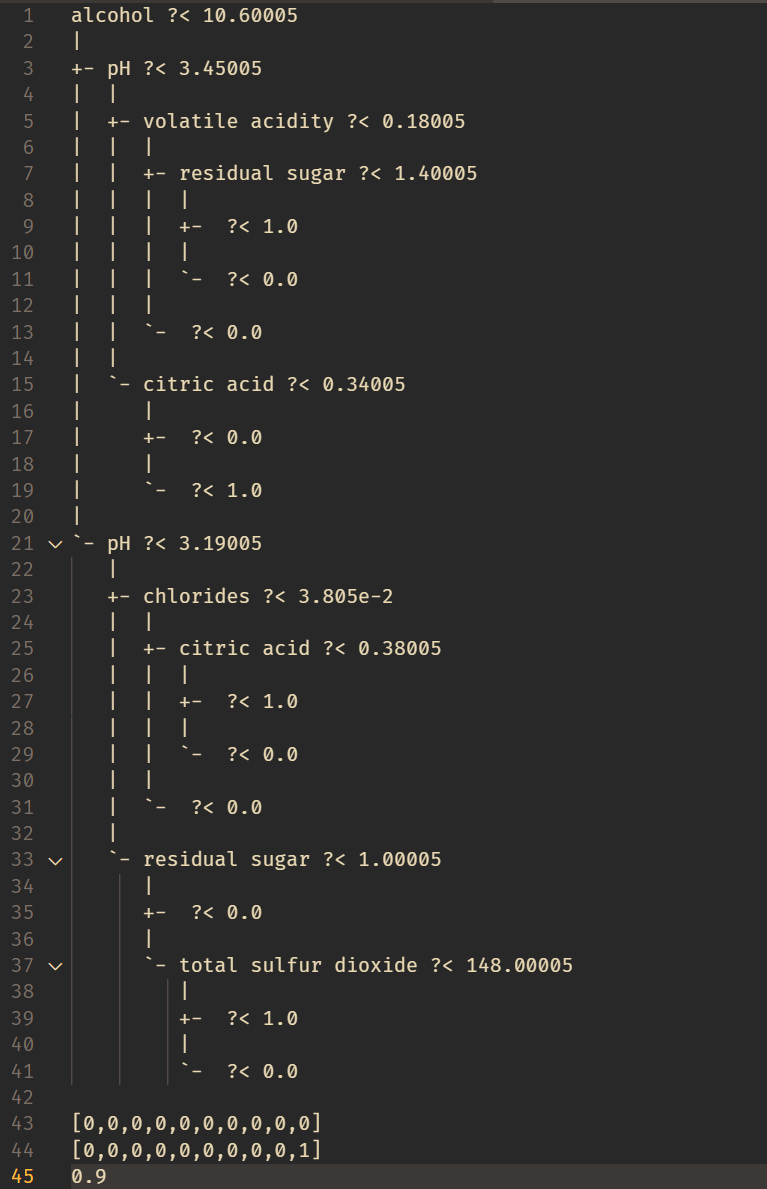
\includegraphics[width=\linewidth]{1.png}
\end{figure}
\end{document}